\documentclass[12pt, oneside]{book}
\usepackage{CU-thesis}

\newcommand{\thesistitleI}{Improving Chest X-ray Diagnostic Classification}
\newcommand{\thesistitleII}{with Transfer Learning and Explainable Deep Learning}
\newcommand{\myname}{Wenxuan Li}

\usepackage{titlesec}
\usepackage{graphicx}
\usepackage{fancyhdr}
\usepackage{longtable}
\usepackage{tocloft}
\usepackage{threeparttable}
\usepackage{booktabs}
\usepackage{fontspec}
\usepackage{pifont}

\newcommand{\circled}[1]{\ding{\numexpr171+#1\relax}}

%%%%%%%%%%%%%%%%%%%%%%%%%%%%%%%%%%%%%%%%%%%%%%%%%
% Define a custom font size for Table of Contents
\newcommand{\tocchapfont}{\fontsize{12}{14}\selectfont\bfseries}
\newcommand{\tocsecfont}{\fontsize{12}{14}\selectfont}
\newcommand{\tocsubsecfont}{\fontsize{12}{14}\selectfont}

\renewcommand{\cftchapfont}{\tocchapfont}
\renewcommand{\cftsecfont}{\tocsecfont}
\renewcommand{\cftsubsecfont}{\tocsubsecfont}
\renewcommand{\cftchappagefont}{\tocchapfont}
\renewcommand{\cftsecpagefont}{\tocsecfont}
\renewcommand{\cftsubsecpagefont}{\tocsubsecfont}
%%%%%%%%%%%%%%%%%%%%%%%%%%%%%%%%%%%%%%%%%%%%%%%%%

\titleformat{\chapter}[display]
  {\normalfont\huge\bfseries}
  {Chapter \thechapter}
  {20pt}
  {\Huge\bfseries}

\titlespacing*{\chapter}{0pt}{50pt}{40pt}

\pagestyle{fancy}
\fancyhf{}
\fancyhead[L]{\leftmark}
\fancyfoot[C]{\thepage}
\renewcommand{\headrulewidth}{0.5pt}
\renewcommand{\footrulewidth}{0pt}

\begin{document}

\frontmatter
\pagestyle{plain}

%%%%%%%%%%%%%%%%%%%%%%%%%%%%%%%%%%%%%%%%%%%%%%
% Title page
\begin{titlepage}
    \begin{center}
        \vspace*{1.0in}

        {\LARGE \textbf{\expandafter{Improving Chest X-ray Diagnostic Classification}}}\\[2mm]
        {\LARGE \textbf{\expandafter{with Transfer Learning and Explainable Deep Learning}}}
        \vfill

        {\scshape by:}\\
        {\large \expandafter{Wenxuan Li}}\\
        \vfill

        {\scshape A Thesis Submitted in Fulfillment of the Requirements\\ for the Degree of}\\[0.25cm]
        \textbf{Bachelor of Science}\\[0.1cm]
        {\scshape in}\\
        \textbf{Computer Science and Technology}\\[0.5cm]

        
\includegraphics[width=0.25\textwidth]{images/university_logo.png}\\[0.5cm]

        {\fontsize{14}{18}\selectfont Department of Computer Science and Technology\\
        Wenzhou-Kean University}\\[0.5cm]
        {\fontsize{14}{18}\selectfont Supervised By: Supervisor's Name}\\[1.5cm]
        {\large \textcopyright{}\fontsize{14}{18}\selectfont June 2026}
    \end{center}
\end{titlepage}

%%%%%%%%%%%%%%%%%%%%%%%%%%%%%%%%%%%%%%%%%%%%
\clearpage

% Info Page
\setcounter{page}{2}
\noindent
Bachelor of Science (2026) \hfill Wenzhou-Kean University\\
Computer Science and Technology \hfill Wenzhou, China
\vspace*{\fill}

\begin{tabular}{l l}
  TITLE:           &\thesistitleI\\
                   &\thesistitleII\\[5mm]
  AUTHOR:          &\myname\\
                   &B.Sc., Computer Science and Technology\\
                   &Wenzhou-Kean University\\
                   &Wenzhou, China\\[5mm]
  SUPERVISORS:     &Dr. Firstname Lastname\\
                   &Enter the name of your second supervisor, if applicable\\[5mm]
  NUMBER OF PAGES: &Fill with the last Roman numeral page of the front matter, \pageref*{endmainmatter}
\end{tabular}

\vfill

%%%%%%%%%%%%%%%%%%%%%%%%%%%%%%%%%%%%%%%%%%%%%%%%
\clearpage
\chapter*{Abstract}
\addcontentsline{toc}{chapter}{Abstract}
This thesis investigates chest X-ray diagnostic classification using deep learning, with a focus on whether transfer learning can improve performance and whether explainable artificial intelligence can improve interpretability. The study uses the NIH ChestXray14 dataset and formulates the task as binary classification, where images labeled ``No Finding'' are treated as normal and images with any pathology label are treated as abnormal. Two convolutional neural network architectures, ResNet50 and DenseNet121, are evaluated under two training settings: training from scratch and transfer learning from ImageNet-pretrained weights. Model performance is assessed using accuracy, precision, recall, F1-score, area under the ROC curve, and confusion-matrix-based error analysis. To improve transparency, Grad-CAM is applied to representative predictions to visualize which image regions influence the model's decisions. Replace this placeholder abstract with the final completed results before submission.

\textbf{Keywords:} chest X-ray classification; transfer learning; deep learning; Grad-CAM; medical image analysis.

\chapter*{Acknowledgements}
\addcontentsline{toc}{chapter}{Acknowledgements}
Replace this section with your final acknowledgements before submission. You may thank your supervisor, readers, family, classmates, and any institution or dataset provider that supported the project.

\clearpage
\tableofcontents

\cleardoublepage
\phantomsection
\listoffigures

\cleardoublepage
\phantomsection
\listoftables

\chapter*{Definition of Acronyms}
\addcontentsline{toc}{chapter}{Definition of Acronyms}
\begin{flushleft}
    \begin{tabular}{|c|l|}
    \hline
    \textbf{Acronym} & \textbf{Definition} \\
    \hline
    AUC & Area Under the Curve \\
    CNN & Convolutional Neural Network \\
    DL & Deep Learning \\
    GPU & Graphics Processing Unit \\
    Grad-CAM & Gradient-weighted Class Activation Mapping \\
    NIH & National Institutes of Health \\
    ROC & Receiver Operating Characteristic \\
    XAI & Explainable Artificial Intelligence \\
    \hline
    \end{tabular}
\end{flushleft}

\chapter*{Definition of Notations}
\addcontentsline{toc}{chapter}{Definition of Notations}
\begin{flushleft}
    \begin{tabular}{|c|l|}
        \hline
        \textbf{Symbol} & \textbf{Meaning} \\
        \hline
        $x$ & Input chest X-ray image \\
        $y$ & Ground-truth class label \\
        $\hat{y}$ & Predicted class label \\
        $p(y=1 \mid x)$ & Predicted probability of the abnormal class \\
        $\mathcal{L}$ & Loss function \\
        $\theta$ & Learnable model parameters \\
        \hline
    \end{tabular}
\end{flushleft}

\mainmatter
\pagestyle{fancy}

\chapter{Introduction}

This thesis studies whether transfer learning and explainable deep learning can improve the performance and interpretability of chest X-ray diagnostic classification. The project is deliberately scoped as a binary classification problem on the NIH ChestXray14 dataset, where images labeled ``No Finding'' are treated as normal and all other labeled cases are treated as abnormal. Two convolutional neural network models, ResNet50 and DenseNet121, are compared under both training-from-scratch and transfer-learning settings, and Grad-CAM is used to visualize the basis of model predictions. The central practical question is not only whether a model can achieve acceptable aggregate metrics, but also whether it can reduce medically important failure cases such as missed abnormal radiographs.

\section{Background}
Chest X-ray imaging is one of the most widely used medical imaging modalities because it is inexpensive, fast, and routinely available in clinical settings. It plays an important role in screening and monitoring thoracic diseases, but manual interpretation can be time-consuming and subject to observer variability. As the number of medical images continues to increase, computer-aided diagnostic systems based on deep learning have become an important research direction. In this context, errors are not equally serious. False positive predictions increase unnecessary follow-up and reduce trust in the system, but false negative predictions are more clinically concerning because an abnormal case may be missed and therefore not receive timely review or further diagnostic attention.

\section{Motivation}
Recent convolutional neural network architectures have shown strong performance in general image recognition and medical image analysis. However, chest X-ray classification still faces practical challenges such as label noise, class imbalance, and limited interpretability. In addition, performance gains reported in the literature often depend on transfer learning, yet the benefit of transfer learning should still be validated in a controlled experimental setting for the selected dataset and task. This motivates a focused comparison between models trained from scratch and models initialized with pretrained weights. It also motivates the use of an explainability method, because a model that appears numerically strong may still be unsuitable for screening if it fails to respond to subtle abnormal findings or attends to irrelevant image regions.

\section{Problem Statement}
The main problem addressed in this thesis is how to build a chest X-ray classification pipeline that is both effective and interpretable. Specifically, this work asks whether transfer learning can improve binary normal-versus-abnormal classification on NIH ChestXray14 and whether Grad-CAM can provide meaningful insight into the prediction behavior of the model. The problem is significant because diagnostic support systems must not only achieve strong quantitative performance but also provide evidence that their decisions are based on medically plausible image regions.

The research gap addressed by this thesis is intentionally narrow. Much of the recent chest X-ray literature emphasizes large multi-label benchmarks, newer architectures, or broad claims about transfer learning, but fewer compact studies isolate a controlled binary normal-versus-abnormal task while directly comparing scratch training, transfer learning, and Grad-CAM-based interpretation across two standard CNN baselines. This thesis addresses that gap through a reproducible capstone-scale comparison rather than through a new model proposal.

\section{Research Objectives}
The objectives of this thesis are as follows:
\begin{itemize}
    \item formulate a clear binary chest X-ray classification task using NIH ChestXray14;
    \item implement two baseline architectures, ResNet50 and DenseNet121;
    \item compare training from scratch against transfer learning for both architectures;
    \item evaluate the models using standard classification metrics and error analysis;
    \item apply Grad-CAM to visualize representative successful and failed predictions.
\end{itemize}

\section{Scope and Limitations}
This study is limited to a single public dataset and a binary classification setting. It does not include lesion localization, segmentation, object detection, federated learning, or clinical deployment. The models are evaluated as research prototypes rather than as medical devices. Interpretability is examined through Grad-CAM, which is useful for qualitative analysis but does not provide a complete explanation of model reasoning.

\section{Research Questions}
This thesis is organized around the following research questions:
\begin{itemize}
    \item How do ResNet50 and DenseNet121 perform on binary chest X-ray classification when trained from scratch?
    \item Does transfer learning improve the performance of these models on\\
    NIH ChestXray14?
    \item What types of prediction errors remain after training, and can Grad-CAM help explain those errors?
\end{itemize}

\section{Thesis Structure}
Chapter 2 reviews prior work on chest X-ray classification, transfer learning in medical imaging, and explainable artificial intelligence. Chapter 3 describes the dataset, preprocessing pipeline, model architectures, training settings, workflow, evaluation metrics, and Grad-CAM method. Chapter 4 presents the experimental setup, quantitative results, training curves, ROC analysis, confusion matrices, and Grad-CAM findings. Chapter 5 integrates the discussion, conclusion, and future-work directions into a single final chapter.

\chapter{Literature Review}

This chapter reviews the main research areas that support the thesis: deep learning for chest X-ray analysis, transfer learning in medical image classification, and explainable artificial intelligence for model interpretation. The purpose of the review is not only to summarize prior work but also to position the present study within a focused and achievable research gap.

\section{Deep Learning for Chest X-ray Classification}
Chest X-ray classification has become a representative application of deep learning in medical imaging because large public datasets have enabled data-driven approaches to disease recognition. Early work in this area established benchmark datasets and demonstrated that convolutional neural networks can detect thoracic abnormalities from chest radiographs. Subsequent studies improved performance through better architectures, training procedures, and label handling strategies. In this section, summarize the major chest X-ray datasets, common classification tasks, and the most influential CNN-based approaches.

\section{ResNet and DenseNet in Medical Imaging}
ResNet and DenseNet are widely used backbones for medical image classification because they balance strong representational power with practical implementation complexity. ResNet introduced residual connections to enable the training of deeper networks, while DenseNet improved feature reuse through dense connectivity. For this thesis, these two architectures are chosen because they are well established, easy to compare, and frequently used in chest X-ray studies. This section should explain why these models are appropriate baselines and summarize how prior medical imaging work has used them.

\section{Transfer Learning in Medical Image Analysis}
Transfer learning is commonly used in medical image analysis because labeled medical datasets are often smaller and noisier than natural image datasets. Initializing a model with weights pretrained on ImageNet can improve optimization, convergence speed, and final performance, especially when the target dataset is limited or imbalanced. However, the magnitude of this benefit depends on the target task, data quality, and fine-tuning strategy. In this section, review studies that compare training from scratch with transfer learning, and explain why this comparison is central to the present thesis.

\section{Explainable Artificial Intelligence for Chest X-ray Models}
High predictive performance alone is insufficient for safety-critical medical applications. Researchers therefore use explainability methods to inspect whether a model attends to clinically meaningful image regions. Among these methods, Grad-CAM is one of the most common because it can visualize class-discriminative regions without major architectural changes. This section should review explainability methods used for chest X-ray classification, discuss their strengths and weaknesses, and clarify why Grad-CAM is an appropriate choice for a compact capstone project.

\section{Research Gap}
Although many studies report strong chest X-ray classification results, fewer present a tightly controlled undergraduate-level study that compares two standard backbones under both scratch and transfer-learning settings and then complements the quantitative results with a focused Grad-CAM analysis. In addition, literature often emphasizes accuracy improvements without equally clear discussion of interpretability and practical error patterns. This thesis addresses that gap through a limited but coherent experimental design centered on one public dataset, one binary task, two architectures, and one explainability method.

\section{Summary}
The literature shows that chest X-ray classification is a mature but still active research area, that transfer learning is often beneficial but should be validated experimentally, and that explainability remains essential for trustworthy model interpretation. Based on these findings, the thesis proceeds with a focused evaluation of ResNet50 and DenseNet121 on NIH ChestXray14, comparing scratch training with transfer learning and interpreting model behavior through Grad-CAM.

\chapter{Methodology}

\section{Research Design}
This thesis adopts a comparative experimental design to evaluate chest X-ray diagnostic classification under a controlled setting. The central goal is to determine whether transfer learning improves binary chest X-ray classification performance and whether explainability methods can make model behavior easier to interpret. To ensure that the comparison is fair, all experiments use the same dataset, label definition, preprocessing pipeline, split strategy, and evaluation metrics. The only differences between the core experiments are the network architecture and the training strategy.

Four main experiments are defined in this study. The first and second experiments use ResNet50, while the third and fourth experiments use DenseNet121. For each architecture, one model is trained from scratch and one model is trained with ImageNet-pretrained weights. This yields the following comparison structure:
\begin{itemize}
    \item ResNet50 trained from scratch;
    \item ResNet50 with transfer learning;
    \item DenseNet121 trained from scratch;
    \item DenseNet121 with transfer learning.
\end{itemize}
This design makes it possible to analyze two questions directly: whether one architecture is more suitable for the selected task, and whether transfer learning provides a consistent performance advantage across both architectures.

\section{System Workflow}
Figure \ref{fig:system-workflow} summarizes the end-to-end workflow used in this thesis. The pipeline begins with NIH ChestXray14 image-label pairs, applies binary label mapping and preprocessing, creates a fixed train-validation-test split, trains the four controlled model configurations, and then evaluates the final models using both quantitative metrics and Grad-CAM-based qualitative analysis. This workflow is intentionally simple so that the full comparison remains reproducible and easy to audit.

\begin{figure}[htbp]
    \centering
    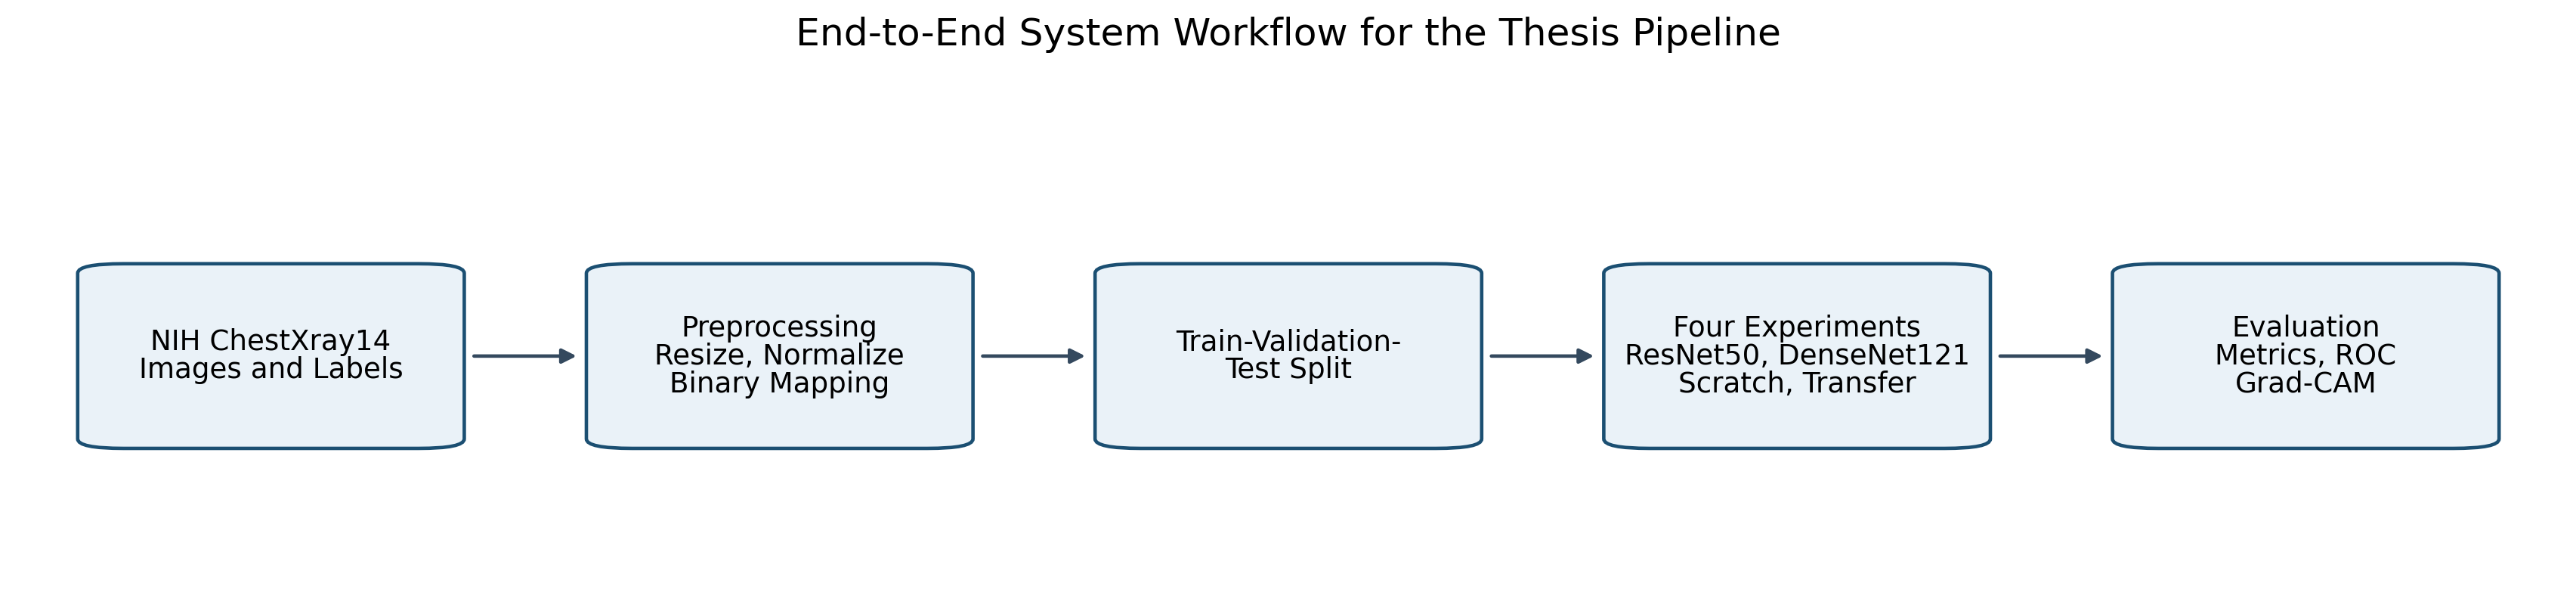
\includegraphics[width=\textwidth]{outputs/figures/thesis_revision/workflow_diagram.png}
    \caption{End-to-end workflow for the thesis pipeline.}
    \label{fig:system-workflow}
\end{figure}

\section{Dataset Description}
The experiments are based on the NIH ChestXray14 dataset, which is one of the most widely used public benchmarks for chest radiograph analysis \cite{ref:wang2017}. The dataset contains a large collection of frontal chest X-ray images with labels mined from radiology reports. Because the original dataset is multi-label and includes several thoracic disease findings, it is useful for many different classification settings. However, for the purpose of this capstone, the task is simplified to binary classification so that the effect of architecture choice, transfer learning, and explainability can be studied in a more controlled way.

In this thesis, all images labeled ``No Finding'' are assigned to the \textit{Normal} class. Images containing one or more pathology labels are assigned to the \textit{Abnormal} class. This mapping converts the original multi-label problem into a binary normal-versus-abnormal decision problem. The binary setting is a practical choice for three reasons. First, it reduces ambiguity in the learning objective. Second, it allows clearer interpretation of evaluation metrics such as sensitivity and specificity. Third, it is appropriate for a focused capstone project where the main goal is comparative analysis rather than full clinical deployment.

This label mapping should be interpreted with caution. The NIH ChestXray14 labels are mined from radiology reports rather than manually annotated for this exact binary task, so label noise is expected. In addition, ``No Finding'' does not necessarily mean that the patient is completely healthy; it only means that no corresponding abnormality was extracted from the associated report. Therefore, the \textit{Normal} and \textit{Abnormal} classes used in this thesis are operational research labels for a controlled experiment, not definitive clinical ground truth.

\section{Data Preprocessing}
The data preprocessing pipeline is designed to produce reproducible model inputs while preserving the overall structure of the chest radiographs. First, metadata are inspected to identify the image path, patient identifier if available, and original disease labels. After the binary label mapping is applied, the dataset is divided into training, validation, and test subsets using a target split ratio of 70\%, 15\%, and 15\%, respectively. If patient identifiers are available, patient-level splitting is used to reduce the risk of data leakage between training and evaluation sets.

All images are resized to $224 \times 224$ pixels so that they can be processed consistently by both ResNet50 and DenseNet121. Since chest X-ray images are grayscale but the selected pretrained models are designed for three-channel input, the image is converted into a model-compatible tensor format while preserving the underlying grayscale information. Pixel values are normalized after resizing so that training remains stable across different model configurations.

To reduce overfitting and improve robustness, training-time augmentation is applied to the training subset only. The final augmentation strategy includes resizing, normalization, and a modest set of geometric or intensity-preserving transformations that do not distort the clinical meaning of the radiograph. The validation and test sets use deterministic preprocessing only, so that the evaluation remains stable and comparable across runs. Every preprocessing step is documented so that the full experimental pipeline can be reproduced later.

\section{Model Architectures}
Two convolutional neural network architectures are used in this study: ResNet50 \cite{ref:he2016} and DenseNet121 \cite{ref:huang2017}. These models are selected because they are well established, widely used in medical image classification, and supported by pretrained ImageNet weights. They also provide a meaningful comparison between two influential design philosophies in convolutional neural networks.

ResNet50 is based on residual learning, where shortcut connections allow information to bypass one or more layers. This helps stabilize optimization in deep networks and makes residual models strong baselines across many vision tasks. In the context of this thesis, ResNet50 is included because it represents a mature and widely adopted architecture that can serve as a reliable benchmark.

DenseNet121 uses dense connectivity, in which each layer receives feature information from earlier layers in the same dense block. This design promotes feature reuse and improves gradient flow during training. DenseNet121 is especially relevant to chest X-ray analysis because it was used by CheXNet and has become one of the most recognizable baselines in this area \cite{ref:rajpurkar2017}. In all experiments, the final classification layer of each network is adapted to output the binary classes required by the selected task.

\section{Training Strategies}
Two training strategies are compared for each model. In the first strategy, the network is trained from scratch using random parameter initialization. In the second strategy, the network is initialized with ImageNet-pretrained weights and then fine-tuned on the target chest X-ray dataset. This comparison is motivated by prior medical imaging work showing that transfer learning often improves convergence and performance when labeled data are limited or noisy \cite{ref:tajbakhsh2016,ref:shin2016}.

The final training configuration used a batch size of 16, a learning rate of $10^{-3}$, the Adam optimizer, and \texttt{BCEWithLogitsLoss} for binary classification. Each experiment was trained for up to 20 epochs, and the best checkpoint was selected based on validation AUC. An early stopping mechanism with patience set to 5 was used to reduce unnecessary computation and to limit overfitting. The same optimization procedure was applied consistently across the four core comparisons.

The same learning rate was used across all experiments to preserve comparability between architectures and training strategies. This design choice keeps the comparison focused on architecture and initialization rather than on separately tuned hyperparameters. However, for pretrained CNN fine-tuning, a lower learning rate can sometimes be more appropriate. Separate learning-rate tuning for scratch and transfer-learning settings is therefore treated as a direction for future work rather than as part of the controlled comparison in this thesis.

For transfer learning, the pretrained model was adapted by replacing the original final classification head with a binary output layer and then fine-tuned on the target dataset under the same experimental conditions used for the scratch-training baseline. Weighted loss was not introduced into the four main comparisons because the goal of the thesis was to preserve a controlled comparison focused on architecture choice and training strategy.

\paragraph{Algorithmic procedure.}
The practical training procedure used throughout the thesis can be summarized as follows:
\begin{enumerate}
    \item Load the predefined training and validation splits and apply the corresponding transforms.
    \item Initialize either ResNet50 or DenseNet121 with scratch weights or ImageNet-pretrained weights.
    \item Replace the original classification head with a binary output layer.
    \item Train the model for one epoch using mini-batch Adam optimization and binary cross-entropy loss.
    \item Evaluate the model on the validation split and record validation AUC.
    \item Save the checkpoint if validation AUC improves; otherwise increment the early-stopping counter.
    \item Stop training when the patience limit is reached or the maximum number of epochs is completed.
\end{enumerate}

\section{Evaluation Metrics}
Model performance is evaluated using a set of standard binary classification metrics. These include accuracy, precision, recall, F1-score, and the area under the ROC curve (AUC). Accuracy measures overall correctness, while precision and recall provide complementary views of positive prediction quality and sensitivity to abnormal cases. F1-score is useful because it balances precision and recall, especially when class distributions are uneven. AUC is included because it measures ranking quality across decision thresholds and is frequently reported in chest X-ray studies \cite{ref:wang2017,ref:irvin2019}.

In addition to these summary metrics, confusion matrices are used to analyze false positives and false negatives. Sensitivity and specificity are also reported because they are especially meaningful in a diagnostic setting. Together, these metrics allow the thesis to compare models not only by final predictive performance but also by error behavior and class-specific tradeoffs.

The binary classification loss used in the experiments is \texttt{BCEWithLogitsLoss}, which combines a sigmoid activation with binary cross-entropy:
\begin{equation}
\mathcal{L} = -\frac{1}{N}\sum_{i=1}^{N} \left[y_i \log \sigma(z_i) + (1-y_i)\log \left(1-\sigma(z_i)\right)\right],
\end{equation}
where $z_i$ is the model logit for sample $i$, $\sigma(\cdot)$ is the sigmoid function, and $y_i \in \{0,1\}$ is the binary class label.

The main evaluation metrics are computed from the standard confusion-matrix counts true positive (TP), true negative (TN), false positive (FP), and false negative (FN):
\begin{equation}
\text{Accuracy} = \frac{TP + TN}{TP + TN + FP + FN},
\end{equation}
\begin{equation}
\text{Precision} = \frac{TP}{TP + FP},
\end{equation}
\begin{equation}
\text{Recall} = \text{Sensitivity} = \frac{TP}{TP + FN},
\end{equation}
\begin{equation}
F1 = \frac{2 \cdot \text{Precision} \cdot \text{Recall}}{\text{Precision} + \text{Recall}},
\end{equation}
\begin{equation}
\text{Specificity} = \frac{TN}{TN + FP}.
\end{equation}
The AUC is not tied to a single decision threshold; instead, it summarizes ranking quality across the full ROC curve by measuring how well abnormal cases are ranked above normal cases.

\section{Explainability with Grad-CAM}
Explainability is incorporated into the methodology through Grad-CAM \cite{ref:selvaraju2017}. After the quantitative evaluation is completed, Grad-CAM is applied to representative images from the test set in order to visualize which image regions most strongly influence model predictions. This process is used for both correctly classified and misclassified cases. By analyzing correct normal predictions, correct abnormal predictions, false positives, and false negatives, the study can examine whether the model focuses on plausible thoracic regions or relies on irrelevant patterns.

The purpose of Grad-CAM in this thesis is not to claim perfect interpretability, but to provide qualitative evidence about model behavior. This is particularly important in medical imaging, where an apparently strong model may still behave unreliably if its predictions are driven by spurious visual cues. Grad-CAM therefore complements the numerical results by supporting a focused error analysis and a discussion of model trustworthiness.

\section{Implementation Environment}
The implementation environment for this study is Python with standard deep learning and data analysis libraries. The core framework is PyTorch, supported by torchvision for pretrained model access and image transforms. Additional tools include NumPy and pandas for data handling, scikit-learn for evaluation metrics, and matplotlib for visualization. Model checkpoints, result tables, training logs, ROC curves, confusion matrices, and Grad-CAM figures are stored in the project workspace so that results can be reused directly in later chapters of the thesis.

Overall, the methodology is designed to balance rigor and feasibility. The project does not attempt to solve every problem in chest X-ray analysis. Instead, it uses a narrow but defensible experimental design to answer a focused research question: whether standard convolutional architectures, combined with transfer learning and Grad-CAM, can provide an effective and interpretable framework for binary chest X-ray diagnostic classification.

\chapter{Experiments and Results}

\section{Experimental Setup}
This section should summarize the final dataset split, preprocessing configuration, hardware environment, and training hyperparameters. It should clearly present the four core experiments so that the reader can understand how the comparison is organized:
\begin{itemize}
    \item ResNet50 trained from scratch;
    \item ResNet50 with transfer learning;
    \item DenseNet121 trained from scratch;
    \item DenseNet121 with transfer learning.
\end{itemize}

\section{Baseline Results}
Present the results of the scratch-training experiments first. This section should include a table containing accuracy, precision, recall, F1-score, and AUC for both architectures. Training curves and confusion matrices may also be included if they help show convergence behavior and major error types.

\section{Transfer Learning Results}
This section should present the results obtained after initializing the models with pretrained weights. The same metrics used in the baseline section should be reported so that direct comparison is possible. The text should note whether transfer learning improves convergence speed, final performance, or both.

\section{Comparative Analysis}
Compare all four experiments in a single integrated discussion. Explain which model performs best overall, which setting is most computationally efficient, and whether transfer learning benefits one architecture more than the other. If the results are mixed, interpret them carefully rather than forcing a simple conclusion.

\section{Grad-CAM Visualization Results}
Present selected Grad-CAM visualizations for representative test cases. Include both correct predictions and failure cases. The discussion should focus on whether the model attends to clinically plausible regions and whether the visualizations help explain common mistakes. This section connects the quantitative results to model interpretability.

\chapter{Discussion, Conclusion, and Future Work}

\section{Interpretation of Results}
This final chapter interprets the experimental findings presented in Chapter 4 and connects them back to the research questions stated in Chapter 1. With all four planned experiments completed, the thesis can compare both architecture choice and training strategy within a single controlled pipeline. This makes it possible to discuss not only the value of pretrained representations, but also the situations in which scratch training may remain competitive.

Across the four experiments, ResNet50 with transfer learning achieved the best overall balance of predictive performance. It produced the highest test accuracy, recall, and F1-score, while DenseNet121 trained from scratch achieved the highest test AUC by a very small margin. DenseNet121 with transfer learning produced lower recall but the highest precision and specificity. This indicates that the architectures and training strategies reached different operating points under the same binary formulation. In practical terms, ResNet50 with transfer learning was better aligned with the screening-oriented objective of reducing missed abnormal cases, while DenseNet121 with transfer learning was stronger at avoiding unnecessary positive predictions.

These findings show that transfer learning is effective for this task, but not in a uniform way. For ResNet50, transfer learning produced clear gains over scratch training across accuracy, recall, F1-score, and AUC. For DenseNet121, however, the scratch model slightly outperformed the transfer-learning model in the main test metrics, while the transfer-learning model became more conservative and achieved higher precision and specificity. This reinforces the thesis claim that architecture choice and training strategy should be evaluated together rather than treated as independent design choices.

\section{Implications for Medical Image Classification}
The results have several implications for practical chest X-ray classification research at the capstone level. First, they show that a relatively focused binary classification problem can still surface meaningful tradeoffs between model architectures. Even when two models achieve similar AUC values, their recall, precision, and specificity can differ substantially. This is important because medical imaging tasks are rarely judged by accuracy alone. In a clinical screening setting, a model that misses too many abnormal images may be less useful even if its overall accuracy remains acceptable.

Second, the Grad-CAM results provide moderate evidence that the selected best-balance model learned clinically plausible spatial patterns. In the correctly classified cases, the heatmaps concentrated mainly on thoracic regions instead of obvious background areas, which supports the claim that the model relied on image content relevant to the chest. This improves the interpretability of the result and makes the model behavior easier to explain in the thesis and in the defense. However, the false positive and false negative examples also demonstrate that plausible visual attention does not guarantee correct reasoning. Grad-CAM should therefore be treated as a transparency tool rather than as proof that the model has learned clinically reliable causal structure.

Third, the completed experiments reinforce the value of keeping the project scope controlled. By restricting the task to chest X-ray binary classification with two architectures and one explainability method, the project was able to produce complete training results, interpretable visual evidence, and a clear comparison that can be defended academically. This is preferable to attempting a much broader medical imaging project that would risk incomplete implementation or weak experimental depth.

\section{Limitations}
Several limitations should be acknowledged when interpreting the final results. The first is dataset quality. NIH ChestXray14 is a widely used public benchmark, but its labels were derived automatically from radiology reports rather than assigned manually for this exact classification task. As a result, label noise is likely present. This limits the confidence with which the measured performance can be interpreted as a true estimate of clinical diagnostic quality.

The second limitation is the binary task formulation itself. In this thesis, all non-``No Finding'' labels were grouped into a single abnormal class. This simplification was useful for making the capstone achievable and for supporting a clean comparison across models, but it also removes important clinical detail. Different abnormalities have different visual signatures and different levels of difficulty. A model that performs reasonably on binary normal-versus-abnormal classification may still struggle on more realistic multi-label or disease-specific tasks.

The third limitation is experimental coverage. Although the full four-way comparison was completed, the project still examines only two model architectures and one binary task formulation. The conclusions therefore should not be generalized to all deep learning approaches for chest X-ray analysis. Additional architectures, alternative thresholds, and disease-specific tasks could reveal different performance patterns.

The fourth limitation concerns explainability. Grad-CAM provides an intuitive visualization of the image regions that most influence the prediction, but it remains a qualitative method. Heatmaps can look plausible even when the underlying prediction is wrong, and different explainability methods may highlight different regions. For this reason, the Grad-CAM analysis in this thesis should be interpreted as supportive evidence about model attention rather than as a definitive account of how the model reasons.

\section{Conclusion}
This thesis investigated whether transfer learning and explainable deep learning could improve chest X-ray diagnostic classification in a focused capstone setting. The study used the NIH ChestXray14 dataset and formulated the task as binary classification, where images labeled ``No Finding'' were treated as normal and images with any pathology label were treated as abnormal. Two convolutional neural network architectures, ResNet50 and DenseNet121, were selected as the main comparison models because both are well established in image classification and have been widely used in medical imaging research. Four controlled experiments were completed in total: ResNet50 from scratch, ResNet50 with transfer learning, DenseNet121 from scratch, and DenseNet121 with transfer learning.

The final experimental results show that the best outcome depends on how performance is defined. DenseNet121 trained from scratch achieved the highest test AUC at 0.7457, while ResNet50 with transfer learning delivered the strongest overall balance of accuracy, recall, and F1-score, reaching a test accuracy of 0.6955, F1-score of 0.6547, and AUC of 0.7454. DenseNet121 with transfer learning produced a similar AUC of 0.7421 and the highest precision and specificity, but at the cost of noticeably lower recall. ResNet50 from scratch served as the weakest of the four runs, with a test AUC of 0.7225. These results indicate that the four configurations reached different tradeoff points under the same binary task formulation, and that transfer learning was clearly beneficial for ResNet50 but not uniformly beneficial for DenseNet121.

The Grad-CAM analysis further supported the practical value of the selected best-balance model. In representative correct predictions, the heatmaps concentrated primarily on thoracic regions rather than on irrelevant image background, suggesting that the model learned clinically plausible visual patterns. At the same time, the false positive and false negative cases showed that plausible attention maps do not guarantee correct decisions. This confirms that explainability should be used to support interpretation of model behavior rather than to replace quantitative evaluation.

Overall, the main implication of this thesis is that a carefully scoped workflow combining controlled experimentation, reproducible evaluation, and explainability can produce academically meaningful results for medical image analysis at the capstone level. Even with a simplified binary problem and only two model architectures, the study was able to reveal clear tradeoffs between sensitivity, specificity, precision, architecture choice, and training strategy. Most importantly, the results show that transfer learning improved ResNet50 substantially, but its benefit was not uniform across architectures. Grad-CAM also improved interpretability by helping connect quantitative model behavior with representative correct and incorrect predictions.

\section{Future Work}
Several directions can extend this work in a more advanced study. First, the binary classification setting can be expanded into multi-label classification so that individual thoracic diseases are modeled directly instead of being merged into a single abnormal class. This would make the task more clinically realistic and allow model performance to be analyzed at the disease level.

Second, the experimental comparison can be broadened. Additional architectures such as EfficientNet, vision transformers, or chest X-ray models trained with self-supervised learning could be evaluated to determine whether the observed ResNet50--DenseNet121 tradeoff generalizes to more recent model families. Future work should also test separate learning-rate schedules for scratch training and transfer-learning fine-tuning, since pretrained models may benefit from a more conservative fine-tuning rate than randomly initialized models. Threshold optimization and calibration should also be explored so that the present accuracy-recall-specificity tradeoffs can be tuned more explicitly for screening or decision-support use cases.

Third, explainability can be improved beyond the present Grad-CAM analysis. Future work could compare Grad-CAM with other explainability methods, incorporate uncertainty estimation, or involve expert review of model heatmaps. This would help determine whether the highlighted regions are not only visually plausible, but also clinically meaningful from a radiological perspective.

Finally, the generalizability of the findings should be tested on additional datasets and settings. External validation on benchmarks such as CheXpert or other institutional chest X-ray collections would provide stronger evidence about robustness across domains. If the long-term goal is clinical deployment or decision support, future work should also examine threshold selection, calibration, domain shift, and user-facing evaluation rather than relying on a single fixed test setting.

\chapter{Conclusion and Future Work}

\section{Conclusion and Implications}
This thesis investigates chest X-ray diagnostic classification using two standard convolutional neural network models, ResNet50 and DenseNet121, under both scratch-training and transfer-learning settings. The study is designed as a focused and reproducible comparison on NIH ChestXray14 using a binary normal-versus-abnormal formulation. In the final version of this section, summarize the quantitative findings, identify the best-performing configuration, and explain whether transfer learning provides a meaningful advantage for this task. You should also state what Grad-CAM reveals about the interpretability of the chosen model and discuss the practical value of combining performance analysis with visual explanation.

\section{Future Work}
Future work can extend this study in several directions. First, the binary classification setting can be expanded to multi-label classification so that individual thoracic diseases are modeled directly. Second, additional architectures such as EfficientNet, vision transformers, or medical-image-specific models can be evaluated. Third, more rigorous explainability and uncertainty estimation methods can be added to complement Grad-CAM. Finally, external validation on other chest X-ray datasets would help assess whether the conclusions generalize beyond the current benchmark.


\begin{thebibliography}{99}
\addcontentsline{toc}{chapter}{References}
\phantomsection
\bibitem{ref:wang2017}
X. Wang, Y. Peng, L. Lu, Z. Lu, M. Bagheri, and R. M. Summers, ``ChestX-ray8: Hospital-scale Chest X-ray Database and Benchmarks on Weakly-Supervised Classification and Localization of Common Thorax Diseases,'' in \textit{Proceedings of the IEEE Conference on Computer Vision and Pattern Recognition}, 2017, pp. 2097--2106.
\bibitem{ref:litjens2017}
G. Litjens et al., ``A Survey on Deep Learning in Medical Image Analysis,'' \textit{Medical Image Analysis}, vol. 42, pp. 60--88, 2017.
\bibitem{ref:he2016}
K. He, X. Zhang, S. Ren, and J. Sun, ``Deep Residual Learning for Image Recognition,'' in \textit{Proceedings of the IEEE Conference on Computer Vision and Pattern Recognition}, 2016, pp. 770--778.
\bibitem{ref:huang2017}
G. Huang, Z. Liu, L. van der Maaten, and K. Q. Weinberger, ``Densely Connected Convolutional Networks,'' in \textit{Proceedings of the IEEE Conference on Computer Vision and Pattern Recognition}, 2017, pp. 4700--4708.
\bibitem{ref:selvaraju2017}
R. R. Selvaraju et al., ``Grad-CAM: Visual Explanations from Deep Networks via Gradient-based Localization,'' in \textit{Proceedings of the IEEE International Conference on Computer Vision}, 2017, pp. 618--626.
\end{thebibliography}

\label{endmainmatter}
\end{document}
